\documentclass{article}


% if you need to pass options to natbib, use, e.g.:
%     \PassOptionsToPackage{numbers, compress}{natbib}
% before loading neurips_2023


% ready for submission
\usepackage[final, nonatbib]{neurips_2023}


% to compile a preprint version, e.g., for submission to arXiv, add add the
% [preprint] option:
%     \usepackage[preprint]{neurips_2023}


% to compile a camera-ready version, add the [final] option, e.g.:
%     \usepackage[final]{neurips_2023}


% to avoid loading the natbib package, add option nonatbib:
%    \usepackage[nonatbib]{neurips_2023}


\usepackage[utf8]{inputenc} % allow utf-8 input
\usepackage[T1]{fontenc}    % use 8-bit T1 fonts
\usepackage{hyperref}       % hyperlinks
\usepackage{url}            % simple URL typesetting
\usepackage{booktabs}       % professional-quality tables
\usepackage{amsfonts}       % blackboard math symbols
\usepackage{nicefrac}       % compact symbols for 1/2, etc.
\usepackage{microtype}      % microtypography
\usepackage{xcolor}         % colors
\usepackage{natbib}

\usepackage{amsmath}
\usepackage{algorithm}
\usepackage[noend]{algpseudocode}
\usepackage[psamsfonts]{amssymb}
\usepackage[pdftex]{graphicx}

% \usepackage{bookmark}

\newcommand{\mbs}[1]{\ensuremath{\boldsymbol{#1}}}
\newcommand{\kv}{\mathbf{k}}
\newcommand{\x}{\mathbf{x}}
\newcommand{\y}{\mathbf{y}}
\newcommand{\z}{\mathbf{z}}
\newcommand{\f}{\mathbf{f}}
\newcommand{\secref}[1]{\hyperref[#1]{Section~\ref{#1}}}
\newcommand{\figref}[1]{\hyperref[#1]{Figure~\ref{#1}}}
\newcommand{\algoref}[1]{\hyperref[#1]{Algorithm~\ref{#1}}}

\newcommand{\K}{\mathbf{K}}
\newcommand{\X}{\mathbf{X}}
\newcommand{\N}{\mathbf{N}}

\newcommand{\IG}{\mathcal{IG}}
\newcommand{\cX}{\mathcal{X}}
\newcommand{\RR}{\mathbb{R}}
\newcommand{\me}{\textup{e}}
\newcommand{\Sigmab}{\mbs{\Sigma}}
\newcommand{\ninit}{n_{\text{init}}}


\title{Practical Bayesian optimization in the presence of outliers}


% The \author macro works with any number of authors. There are two commands
% used to separate the names and addresses of multiple authors: \And and \AND.
%
% Using \And between authors leaves it to LaTeX to determine where to break the
% lines. Using \AND forces a line break at that point. So, if LaTeX puts 3 of 4
% authors names on the first line, and the last on the second line, try using
% \AND instead of \And before the third author name.


\author{%
  Thomas Gaviard\\
  Code available online at \url{https://github.com/tms-gvd/project_bl}\\
  \texttt{thomas.gaviard@centrale.centralelille.fr}
}


\begin{document}


\maketitle

\begin{abstract}
  Bayesian optimization is a powerful tool for optimizing black-box functions. However, it is known to be sensitive to outliers. In this report, I present my study of the paper \textit{Practical Bayesian optimization in the presence of outliers} by \cite{martinez-cantinPracticalBayesianOptimization2017} that proposes a new algorithm to filter outliers during the optimization.
\end{abstract}


\section{Settings}

The authors study \textbf{sample efficient optimization} that is a common task in many fields. It consists of minimizing a function $f : \cX \subset \RR^d \rightarrow \RR$ that is expensive to evaluate. For instance, $f$ can be the error rate of a machine learning classifier model trained with a given set of hyperparameters. Then, the goal would be to find the hyperparameters that minimize a metric. Yet, evaluating $f$, i.e. training the model, is expensive and time-consuming that is why we want to minimize the number of evaluations of $f$.

\textbf{Bayesian optimization} (BO) is a powerful method for sample efficient optimization as it provides a black-box solution. To this end, it uses a probabilistic surrogate model of the function $f$ that is cheap to evaluate and leverages the data observed so far during the optimization. This "memory" helps to sample efficiently and yields great performance.

The optimization is performed as follows:
\begin{itemize}
  \item \textbf{Initialization:} Draw $p$ samples at random from $\cX$ and evaluate $f$ at these points.
  \item \textbf{For $t = 1, \dots, T$:}
  \begin{itemize}
    \item Use the previously observed data $\y=\y_{1:t}$ at points $\X=\X_{1:t}$ to fit a surrogate model $s_t$ of $f$. 
    \item The next point to evaluate $\x_{t+1}$ is selected by optimizing an \textit{acquisition function} over $\cX$.
    \item Finally, evaluate $f$ at $\x_{t+1}$ and add the new observation $y_t$ to $\mathcal{D}_t$.
  \end{itemize}
\end{itemize}

The paper restricts their study to the expected improvement (EI) for the acquisition function, which is defined as follows:
\begin{equation}
	\label{eq:ei}
	EI(\x) = \mathbb{E}_{p(y|s_t(\x))} \left[\max(0,y^* - y)\right],
\end{equation}
where $y^*=\max(y_1,\ldots,y_t)$.

The authors assume that the data is observed under homoscedastic noise, i.e. $y_i = f(\x_i) + \epsilon_i$ where $\epsilon_i \sim \mathcal{N}(0, \sigma_n^2)$. Then, they choose to use a \textbf{Gaussian Process} (GP) for the surrogate model $s_t$ as it is a common choice. They consider a zero-mean GP with covariance $k : \cX \times \cX \rightarrow \RR$. Therefore, the likelihood can be written as $y | f \sim \mathcal{N}(f, \sigma_n^2)$ where $f \equiv f(\x)$. A common choice will be to use a \textbf{Gaussian likelihood} which leads to a closed-form expression for the posterior distribution.

Yet, the authors also assume that the data can contain \textbf{outliers}. For the previous example of the machine learning model, an outlier could be a model that is not trained properly due to random bugs, I/O errors, convergence issues for some hyperparameters sets, etc. Nevertheless, BO is known to be sensitive to these outliers because of its "memory" component.

Particularly, the Gaussian likelihood is not robust to outliers. Indeed, the Gaussian distribution has light tails, i.e. it assigns low probability to events that are far from the mean. Therefore, the posterior distribution will be strongly influenced by outliers. To overcome this issue, the authors propose to use a \textbf{Student-t likelihood} that has heavier tails. This means that it assigns more probability to events that are further from the mean. Thus, the posterior distribution will be less influenced by outliers.

\section{Contributions}

% The contribution of the paper is to propose a new algorithm \algoref{al:robustbo} to filter outliers during the optimization process. To this end, they use a GP with a Student-t likelihood (\verb+fitGPwithTlik+) that is more robust to outliers than a Gaussian one. This GP is used to filter the points that were evaluated and considered as outliers (\verb+filterOutliers+). Then, the optimization is performed on the filtered data with a GP with a Gaussian likelihood (\verb+fitGPwithGlik+).

\begin{algorithm}
  \renewcommand{\algorithmicrequire}{\textbf{Input:}}
  \caption{BO with outliers\label{al:robustbo}}
  \begin{algorithmic}[1]
    \Require Total budget $T$, rejection threshold $\alpha$ 
    \State Initial design of $p$ points (e.g.: LHS)
     \Statex \hspace{\algorithmicindent} $\X~\gets~\x_{1:p} \qquad  \y \gets y_{1:p}$
  \Statex
  \For{$t = p+1 \ldots T$}
   \If {schedule($t$)}
     \State $\mathbf{\Theta_t} \gets \text{fitGPwithTlik}(\X,\y)$
     \State $\X_{in}, \y_{in} \gets \text{filterOutliers}(\X,\y,\mathbf{\Theta_t}, \alpha)$
   \EndIf
     \Statex
     \If {$length(\y_{in}) < \lfloor length(\y) / 2 \rfloor$ \textbf{or} \\\hspace{\algorithmicindent} \textbf{not} schedule($t$)}
     \State $\X_{in} \gets \X \qquad  \y_{in} \gets \y$
     \EndIf
     \Statex
     \State $\mathbf{\Theta_g} \gets \text{fitGPwithGlik}(\X_{in}, \y_{in})$ 
     \State $\x_t = \arg\max_{\x} \; EI(\x | \X_{in}, \y_{in},\mathbf{\Theta_g})$
     \State $y_t \gets f(\x_t) \qquad \X \gets add(\x_{t}) \qquad  \y \gets add(y_{t})$
  \EndFor
  \end{algorithmic}
\end{algorithm}

I will present two aspects of the paper. First, I will re-derive the form of the posterior distribution with a Student-t likelihood and the Laplace approximation. Then, I will test the proposed strategy of the paper on simple examples.


\section{Derivation of Laplace approximation for the Student-t Process}

Reminder that for a GP with a Gaussian likelihood, the posterior distribution is in closed-form and the predictions at a query point $\x_q$ follows a Gaussian distribution with parameters:
\begin{equation}
  \label{eq:predgp}
  \begin{split}
    \mu(\x_q) &= \kv(\x_q,\X)^T\K^{-1}\y, \\
    \sigma ^2 (\x_q) &= k(\x_q, \x_q) - \kv(\x_q,\X)^T \K^{-1} \kv(\x_q,\X),    
  \end{split}
\end{equation}
where
\begin{equation}
  \label{eq:covmatrix}
  \begin{split}
	\kv(\x_q,\X) &= \begin{pmatrix}k(\x_q,\x_1) &\ldots& k(\x_q,\x_t)\end{pmatrix}^T\!, \\
  \K &= \begin{pmatrix}\kv(\x_1,\X) &\ldots& \kv(\x_t,\X)\end{pmatrix} + \mathbf{I}\sigma^2_n.    
  \end{split}
\end{equation}

In the paper, the authors use a Mat\'ern kernel with $\nu = 5/2$.

The authors use the following definition of the Student-t likelihood, with $f \equiv f(\x)$.
\begin{equation}
	\label{eq:likt}
	t(y;f,\sigma_0,\nu) = \frac{\Gamma\left(\nu + \frac{1}{2}\right)}{\Gamma(\frac{\nu}{2}) \sqrt{(\nu\pi)\sigma_0}}\left[1+\frac{(y-f)^2}{\nu\sigma_0^2}\right]^{-(\nu + 1) / 2},
\end{equation}

The Laplace approximation for the conditional posterior of the latent function, which we write as $q(\f | \y, \X) \approx p(\f | \y, \X)$ with $\f = \left( f (\x_i) \right)_{1 \leq i \leq t}$, is constructed from the second order Taylor expansion of log posterior around the mode $\hat{\f} = \arg\max_\f p(\f | \y, \X)$:
\begin{equation*}
  \log p(\f | \y, \X) = \log p(\hat{\f} | \y, \X)
    + \frac{1}{2} (\f - \hat{\f})^T \ \nabla \nabla_\f \log p(\f | \y, \X) |_{\f = \hat{\f}} \ (\f - \hat{\f}) + o(||\f - \hat{\f}||^2)
\end{equation*}
as $\nabla_\f \log p(\f | \y, \X) |_{\f = \hat{\f}} = 0$.

This can be simplified as follows keeping only the terms that depends on $\f$:
\begin{equation*}
  \log q(\f | \y, \X) = - \frac{1}{2} \ (\f - \hat{\f})^T \ \Sigmab_{\text{LA}}^{-1} \ (\f - \hat{\f}) + \text{const}
\end{equation*}
with $\Sigmab_{\text{LA}}^{-1} = - \nabla \nabla_\f \log p(\f | \y, \X) |_{\f = \hat{\f}}$.

We recognize that:
\begin{equation*}
  q(\f | \y, \X) \propto \exp \left( - \frac{1}{2} \ (\f - \hat{\f})^T \ \Sigmab_{\text{LA}}^{-1} \ (\f - \hat{\f}) \right)
\end{equation*}
meaning that the Laplace approximation of $\f | \y, \X \sim \mathcal{N}(\hat{\f}, \Sigmab_{\text{LA}})$.

Using $p(\f | \y, \X) \propto p(\y | \f, \X) \ p(f | \X)$, we simplify $\Sigmab_{\text{LA}}$ as follows keeping only the terms that depends on $\f$:
\begin{align*}
  \log p(\f | \y, \X) &= \log p(\y | \f, \X) + \log p(\f | \X) \\
  &= \log p(\y | \f, \X) + \left( - \frac{1}{2} \ \f^T \ \K^{-1} \ \f \right) \; \text{as $\f | \X \sim \mathcal{N}(0, \K)$ by definition of the GP}\\
\end{align*}

Using $- \nabla \nabla_\f \left( - \frac{1}{2} \ \f^T \ \K^{-1} \ \f \right) = K^{-1} $, we can rewrite $\Sigmab_{\text{LA}}^{-1} = \mathbf{W} + \K^{-1}$ with $\mathbf{W} = - \nabla \nabla_\f \log p(\y | \f, \X) |_{\f = \hat{\f}}$. $\mathbf{W}$ is diagonal since the likelihood factorizes over the data points, i.e. the distribution for $y_i$ depends only on $f_i$.

Eventually, the likelihood follows a Student-t distribution then keeping only the terms that depends on $\f$:
\begin{align*}
  - \log p(y_i | f_i, \x_i) &= \frac{\nu + 1}{2} \ \log \left( 1 + \frac{(y_i - f_i)^2}{\nu \sigma_0^2}\right) \\
  - \nabla \nabla_\f \log p(y_i | f_i, \x_i) = \mathbf{W}_{i, i} &= - (\nu + 1) \ \frac{r_i^2 - \nu \sigma_0^2}{(r_i^2 + \nu \sigma_0^2)^2}
\end{align*}
with $r_i = y_i - f_i$.

To make \textbf{predictions}, we need to compute the posterior distribution $p(f_q | \y, \X, \x_q)$. With the Laplace approximation, we have:
\begin{align}
  \mathbb{E}_q [f_q | \X, \y, \x_q] &= \int \mathbb{E}_q [\f | \X, \y, \x_q] p(\f | \X, \y) d\f \nonumber \\
  &= \int \mathbf{k}(\x_q, \X)^T \K^{-1} \f \ p(\f | \X, \y) d\f \nonumber \\
  &= \mathbf{k}(\x_q, \X)^T \K^{-1} \mathbb{E} [\f | \X, \y] \nonumber \\
  &=  \mathbf{k}(\x_q, \X)^T \K^{-1} \hat{\f}
\end{align}
Similarly, we get a closed-form expression for the variance:
\begin{equation}
  \mathbb{V}_q [f_q | \X, \y, \x_q] = k(\x_q, \x_q) - \mathbf{k}(\x_q, \X)^T \left(K + W^{-1}\right)^{-1} \mathbf{k}(\x_q, \X)
\end{equation}

For a given $\X, \y$, the mode $\hat{\f}$ can be computed using the expectation maximization (EM) algorithm as detailed in \cite{NIPS2009_13fe9d84}.

\section{Experiments}

Firstly, I implemented the Gaussian Process with Student-t likelihood using Laplace approximation and check that it works as expected. Secondly, I implemented the proposed \algoref{al:robustbo} and tested it on simple examples.

\subsection{Gaussian Process with Student-t likelihood}

To check that the implementation of GP with Student-t likelihood works as expected, I generated two simple datasets with outliers. The first one is the 1D Forrester function defined as follows:
\begin{equation}
  \label{eq:forrester}
  f(x) = (6x - 2)^2 \sin(12x - 4)
\end{equation} on the support $x \in [0, 1]$.

The second one is the 2D Branin function defined as follows:
\begin{equation}
  \label{eq:branin}
  f(x_1, x_2, l) = \left(x_2 - \left( \frac{5.1}{4 \pi^2} - 0.1 (1 - l)\right)x_1^2 + \frac{5}{\pi} x_1 - 6 \right)^2 +
    10 (1 - \frac{1}{8 \pi}) \cos(x_1) + 10
\end{equation} on the support $x_1 \in [-5, 10], x_2 \in [0, 15]$ with $l \in \{0, 1\}$ the degree of fidelity.

I compared the implementation with 3 other GPs:
\begin{itemize}
  \item GP with Gaussian likelihood, without outliers
  \item GP with Gaussian likelihood, with outliers
  \item GP with Student-t likelihood, computed using \textrm{ApproximateGP} with Variational Inference from \textrm{GPyTorch}.
\end{itemize}

\begin{figure}[ht]
  \centering
  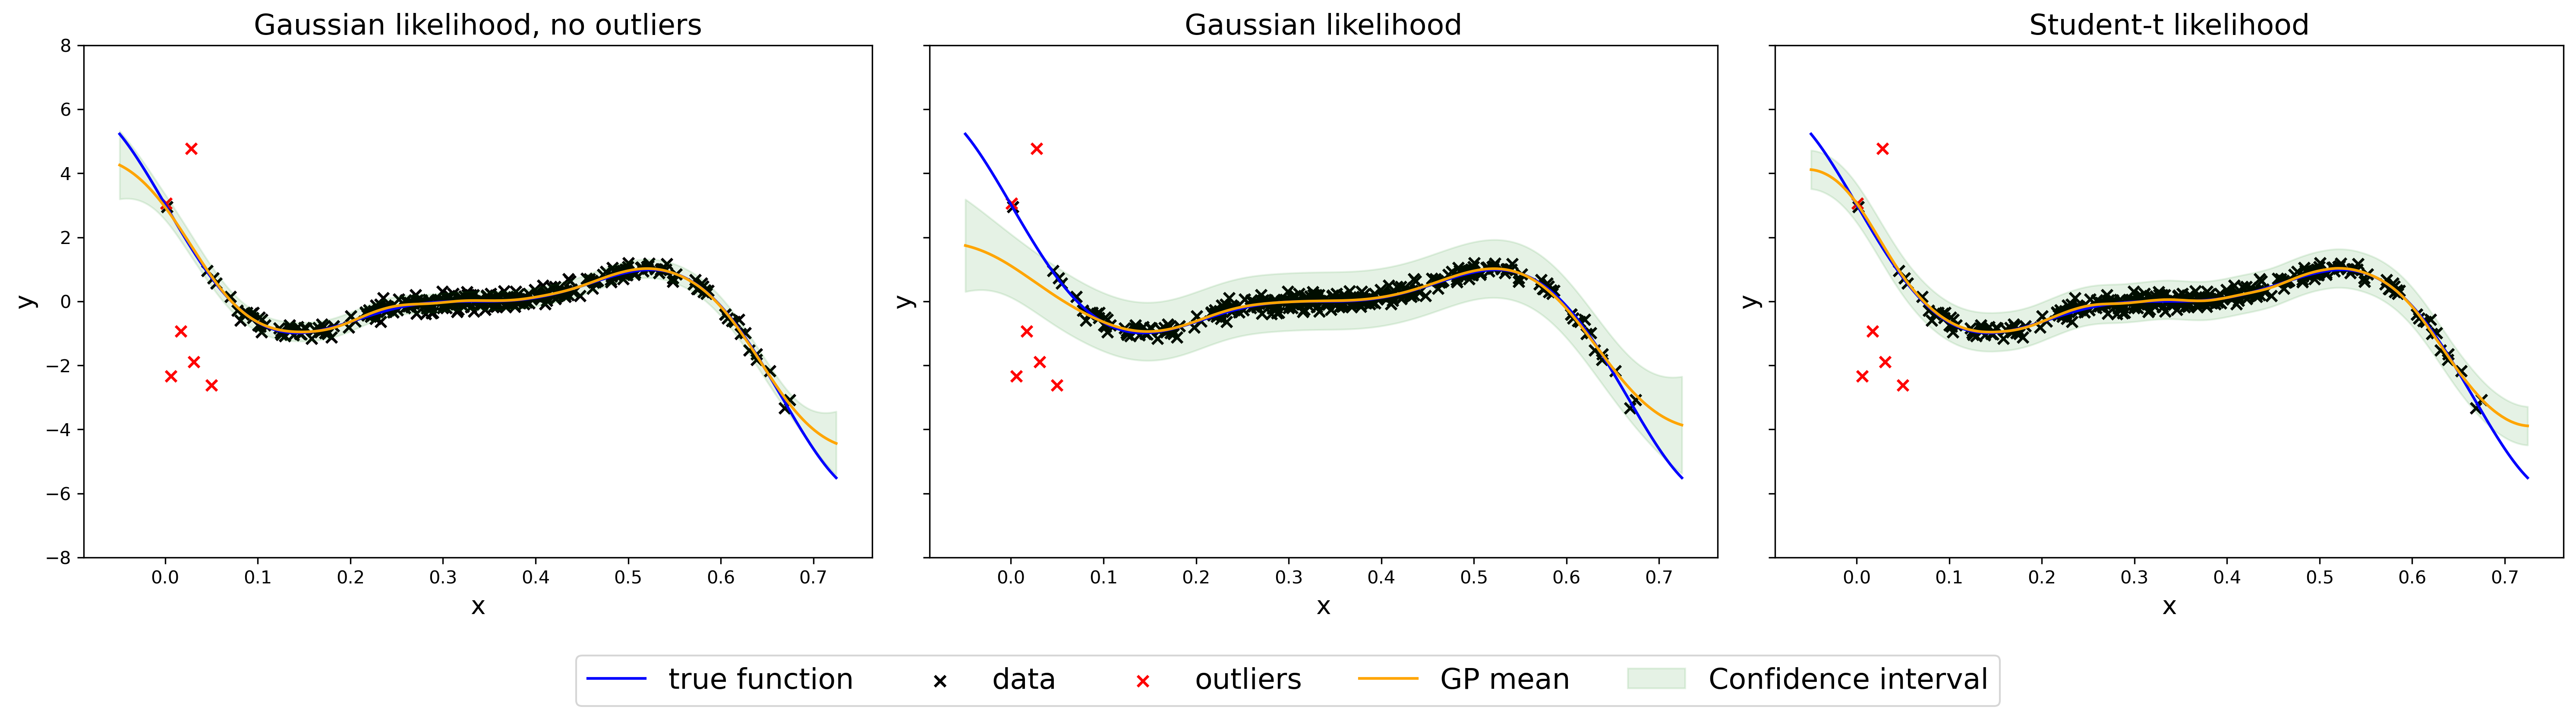
\includegraphics[width=\linewidth]{imgs/gp_1d.png}
  \caption{GP for different likelihoods in the presence or not of outliers, for the Forrester function. Points that were generated as outliers are represented in red.}
  \label{fig:gp_1d}
\end{figure}

\begin{figure}[ht]
  \centering
  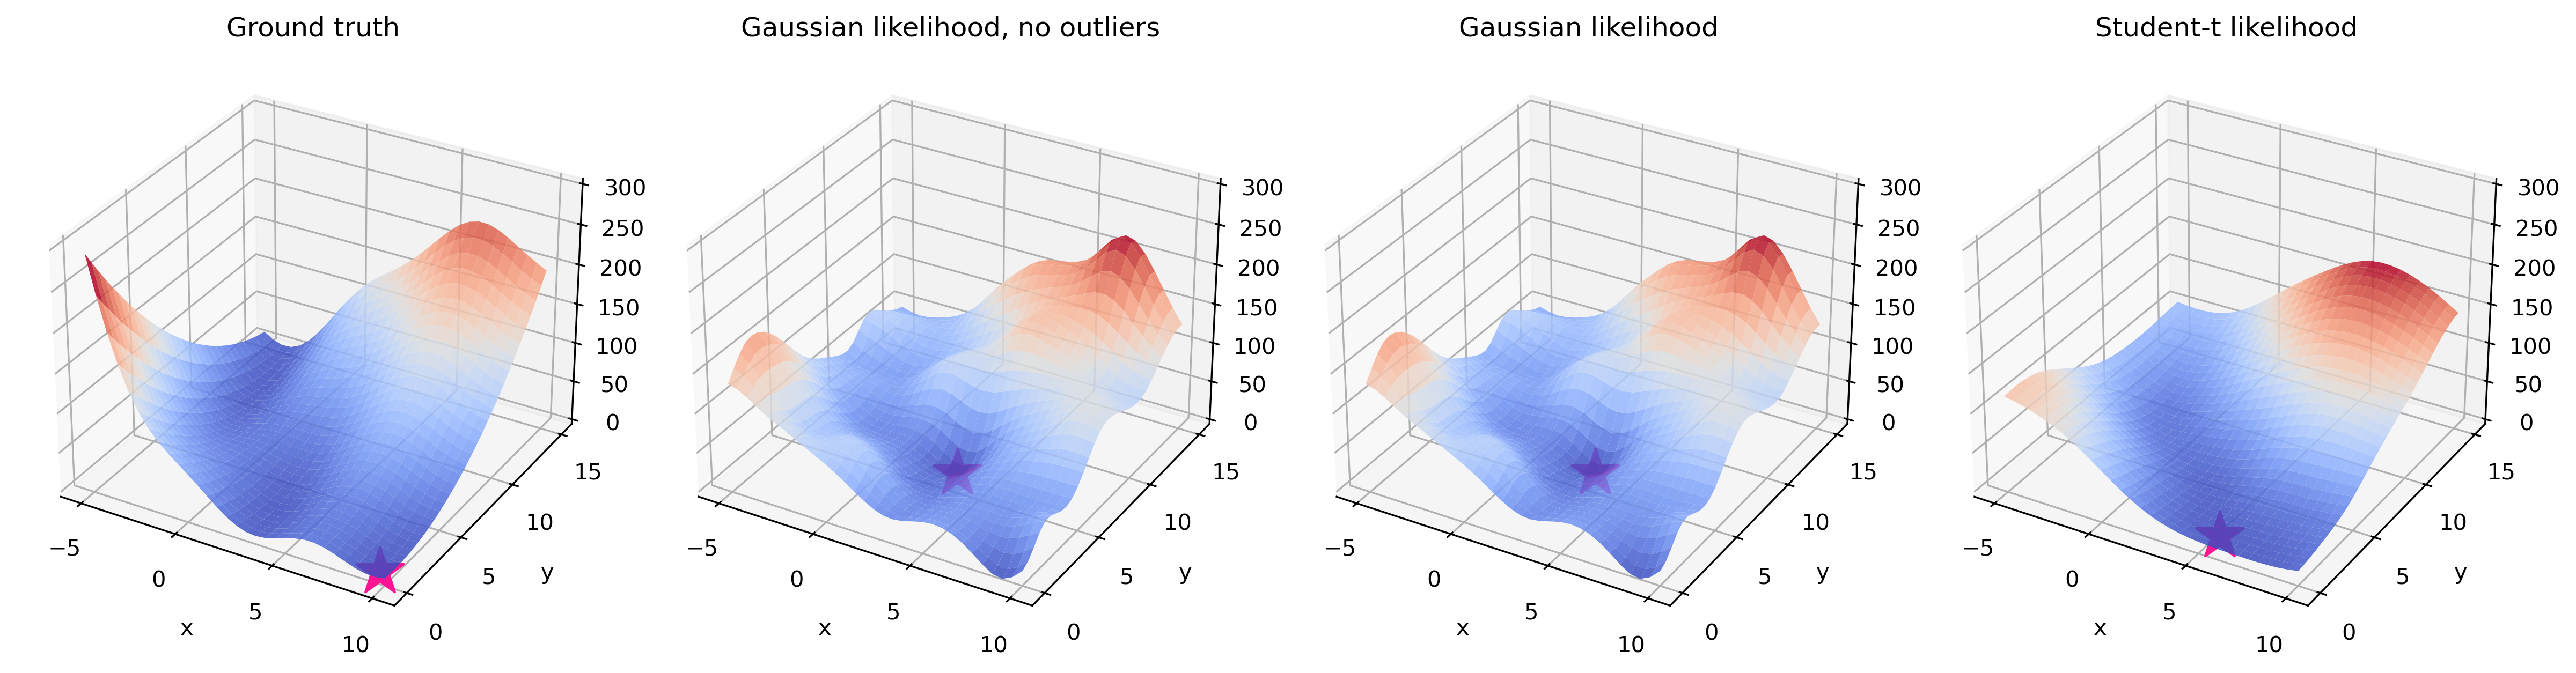
\includegraphics[width=\linewidth]{imgs/gp_2d.png}
  \caption{GP for different likelihoods in the presence or not of outliers, for the Branin function with $l=0.8$. The pink star shows the minimum of the function.}
  \label{fig:gp_2d}
\end{figure}

\ref{fig:gp_1d} and \ref{fig:gp_2d} show that the GP with Student-t likelihood is more robust to outliers than the GP with Gaussian likelihood. For the 1D example, the GP with Student-t likelihood is less influenced by the outliers in [0, 0.1] and the confidence interval is tighter on the whole domain than with a Gaussian likelihood. This even more noticeable for the 2D case.

To compute the GP with Student-t likelihood, I implemented the EM algorithm to get $\hat{\f}$ and $\mathbf{W}$ as detailed in \cite{NIPS2009_13fe9d84}. I also implemented the Laplace approximation to compute the posterior distribution $p(f_q | \y, \X, \x_q)$. Yet, I did not finish the last part that was to optimize the hyperparameters. According to the previous paper, $p(\theta | \y, \X)$ is differentiable with respect to $\theta$ and can be optimized using gradient descent. I believe that it can be done by writing a custom likelihood in \textrm{GPyTorch} using $\hat{\f}$ and $\mathbf{W}$.



\subsection{Bayesian optimization with Student-t likelihood to filter outliers}

Using the previous implementation of GP with Student-t likelihood, I implemented the proposed \algoref{al:robustbo} and tested it on the Forrester function and the Branin function with $l=0.8$. I used the same acquisition function as in the paper, i.e. the expected improvement (EI) defined in \eqref{eq:ei}. I did not tested it in higher dimension as the time to compute $\arg \max_{\x} \; EI(\x | \X_{in}, \y_{in},\mathbf{\Theta_g})$ grows exponentially with the dimension if we compute it naively by sampling points and evaluating the acquisition function at each point. Yet, as $EI$ is differentiable with respect to $\x$, we can use gradient descent to optimize it. Yet, the function is not striclty convex and on the contrary has many local minima. Therefore, we need to use a good initialization to avoid getting stuck in a local minimum. Even though I did not have time to implement it, it is feasible thanks to \textrm{BoTorch} as they explain how to do it in this \href{https://botorch.org/v/0.1.2/tutorials/optimize_stochastic}{tutorial}. The main idea is to choose a good initialisation to converge to the global minimum by sampling promising points and leveraging parallel computing.

I created animated gifs to show the optimization process for the Forrester function and the Branin function with $l=0.8$.
They are available online at \href{https://github.com/tms-gvd/project_bl/blob/main/1d_bo.gif}{1D BO} and \href{https://github.com/tms-gvd/project_bl/blob/main/2d_bo.gif}{2D BO}. We can observe that the filter is efficient to remove outliers like the outlier at (-0.7, 10) at the ninth iteration for the Forrester function. The oscillations between two states for the Branin function comes to the fact that we fit a Student-t GP every two steps. Then, it filters a lot of outliers and keep the most promising points that emphasize the area that we look at.

In addition, I studied the impact of two parameters for the Forrester function. Firstly, the impact of the rejection threshold $\alpha$ that is the threshold to consider a point as an inlier. It is computed as folows: all points that fall in the $\alpha$-percentile are considered as outliers. The higher $\alpha$ is, the more points are considered as outliers. \figref{fig:alpha} presents the evolution of $f(x_{best}) - f(x^*_t)$ during the optimization. We observe that extreme values for $\alpha$ are not efficient. Indeed, if $\alpha$ is too low, we do not filter enough outliers and the optimization is not robust. On the contrary, if $\alpha$ is too high, we filter too many points and the optimization is not efficient either, mostly because of the second if condition in the algortithm that says that there are at least half points that are inliers and if it is not the case during the BO, then it shoudl be a mistake and we take all the points as inliers for the current step.

Secondly, I studied the impact of the probability of outliers generated. Indeed, the outliers are generated randomly with a probability $p_{out}$. \figref{fig:ninit} presents the evolution of $f(x_{best}) - f(x^*_t)$ during the optimization. We observe that the optimization is not robust to outliers if $p_{out}$ is too high. It is relevant as in this case we generate too many outliers and the optimization is not robust. In addition, too many outliers can mislead the GP, even with Student-t likelihood.

\begin{figure}[ht]
  \centering
  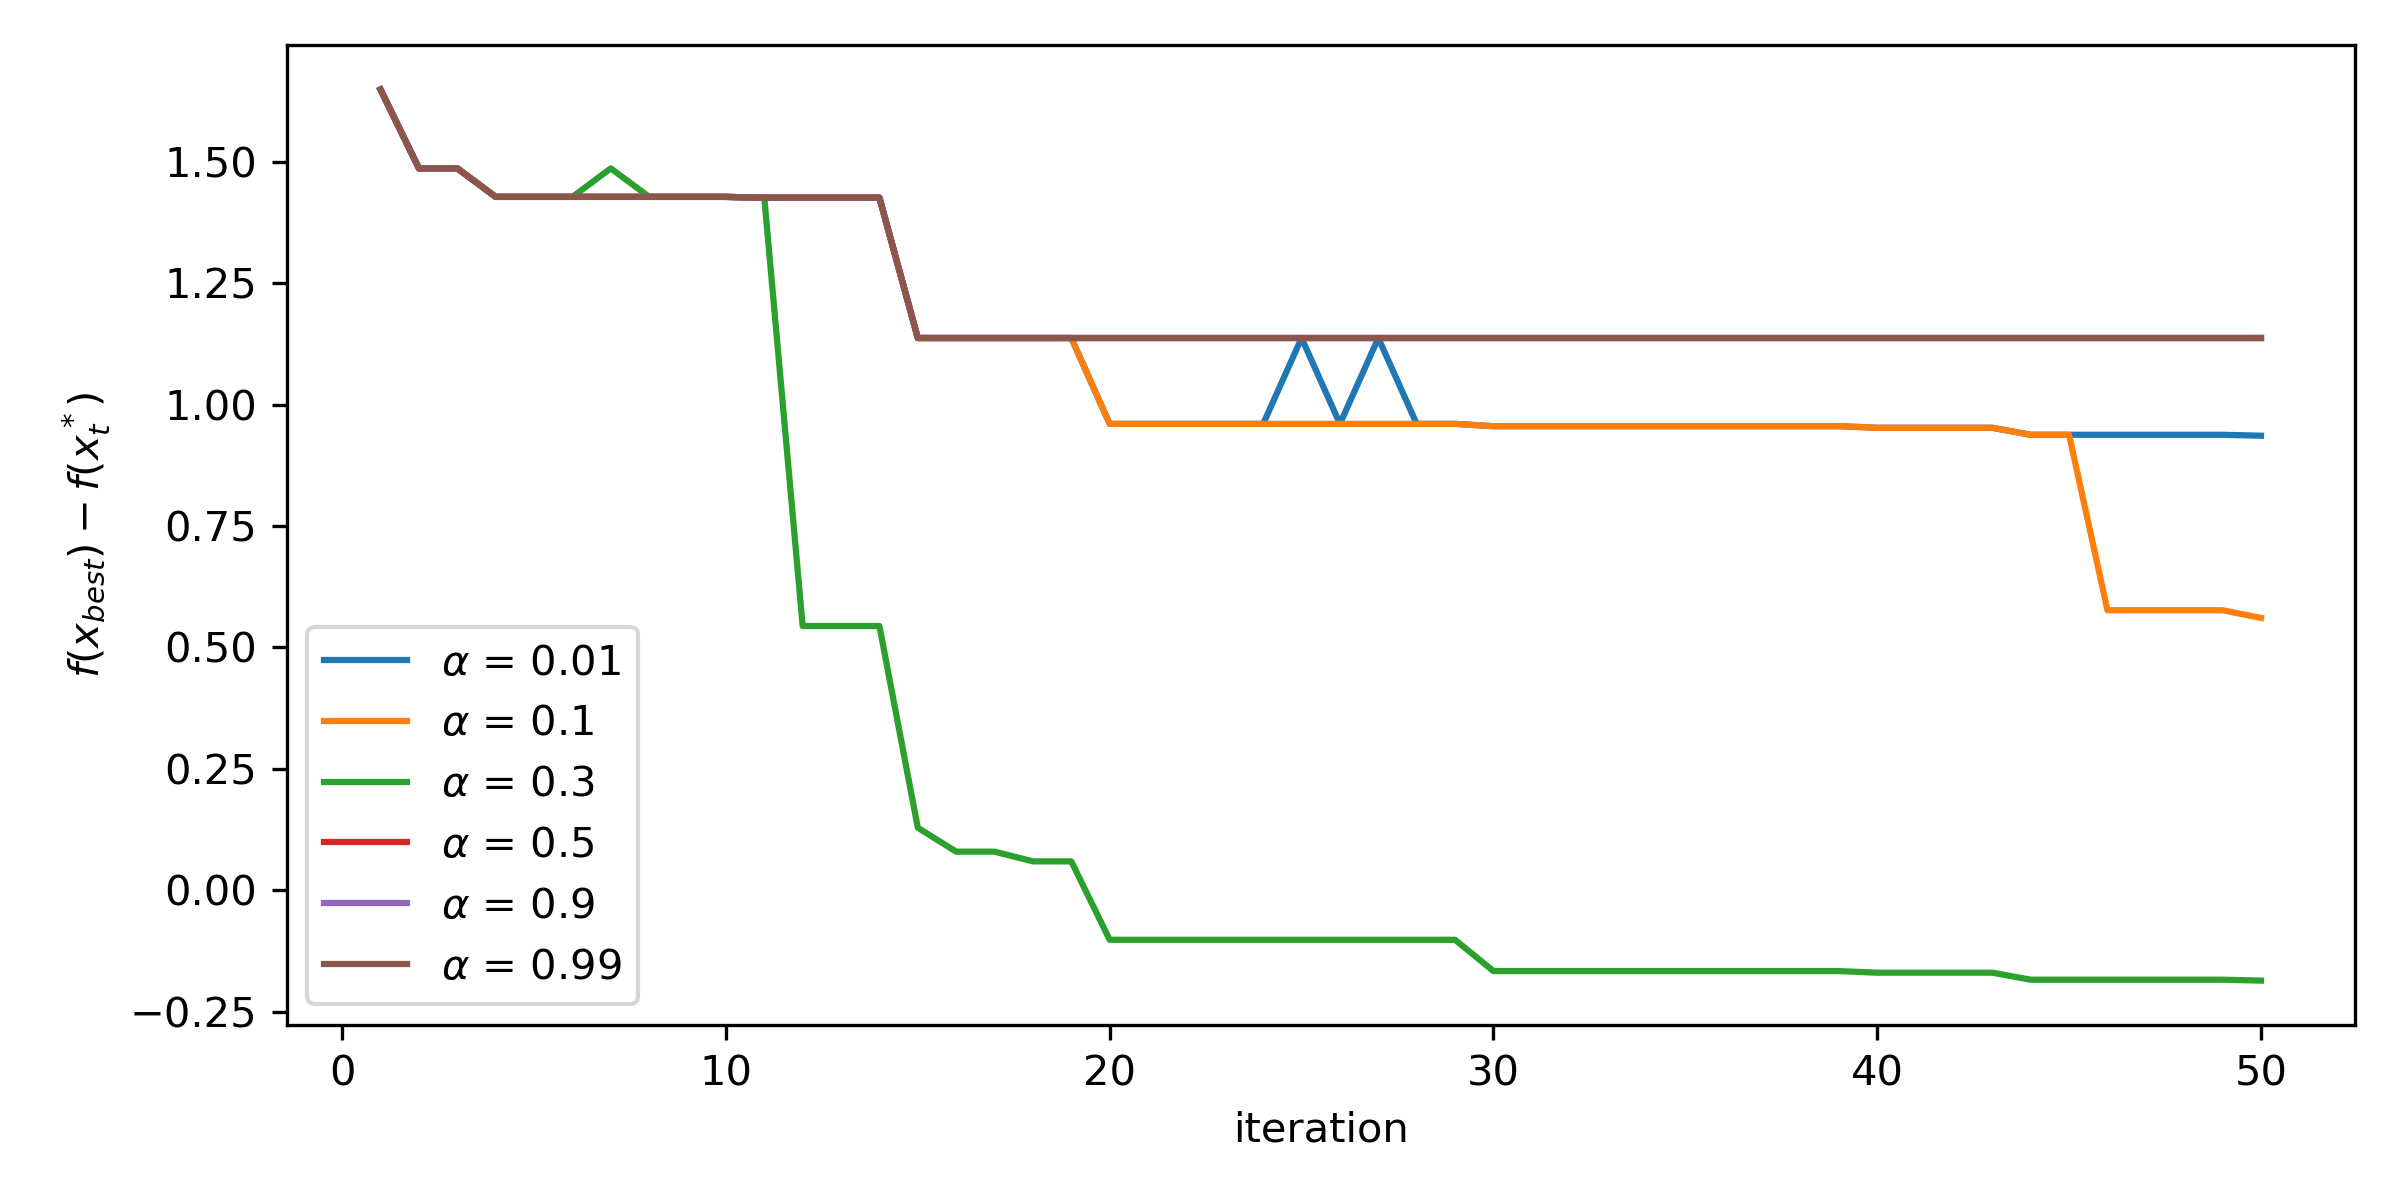
\includegraphics[width=.8\linewidth]{imgs/alpha.png}
  \caption{Impact of the rejection threshold $\alpha$ on the BO for the Forrester function.}
  \label{fig:alpha}
\end{figure}

\begin{figure}[ht]
  \centering
  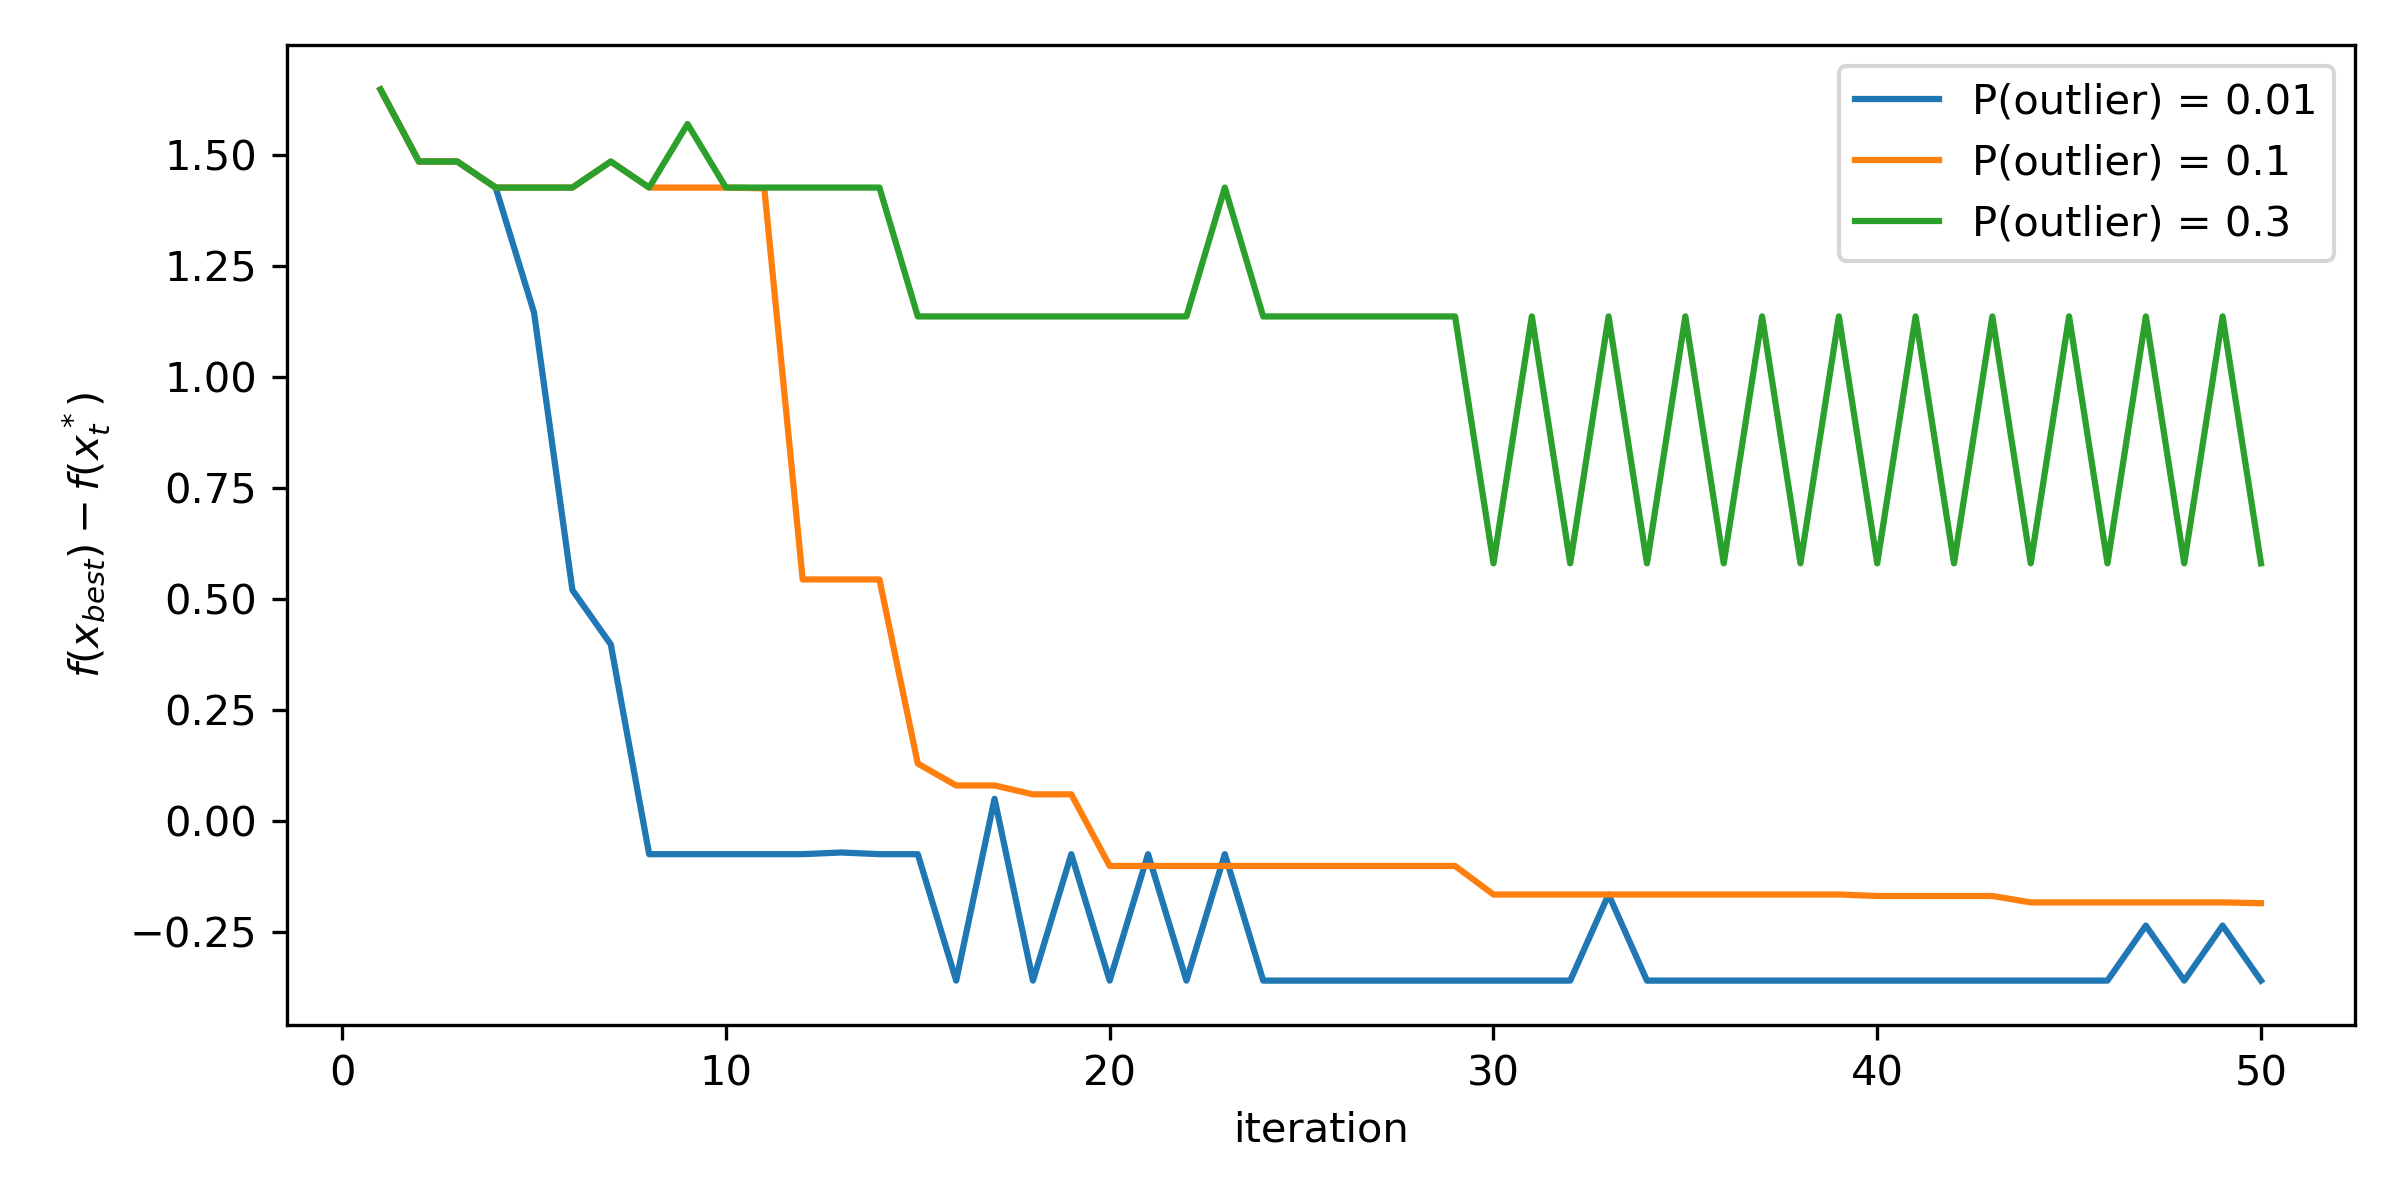
\includegraphics[width=.8\linewidth]{imgs/prob_out.png}
  \caption{Impact of the probability of outliers generated on the BO for the Forrester function.}
  \label{fig:ninit}
\end{figure}

\bibliography{BL}
\bibliographystyle{apalike}

%%%%%%%%%%%%%%%%%%%%%%%%%%%%%%%%%%%%%%%%%%%%%%%%%%%%%%%%%%%%


\end{document}